%
\documentclass[../template.tex]{subfiles}
\usepackage{graphicx}

\begin{document}

%Maze pag. 100 to do

\section{General Absorbing Markov Chain}
Consider some kind of metric $g(X)$, as a function mapping each \textbf{transient state} to a real number. We suppose that every time the chain visits a state $j$, the metric rises by the value of $g(j)$. In other words, $g(j)$ is the \q{reward} earned by the process by visiting $j$.

As before, we label all states so that the first $r$ are transient, and the last $N-r$ are absorbing.

Denoting with $T$ the absorption time for a process starting in state $i$. The average \textit{cumulative} value of the metric is given by:
\begin{align*}
    w_i = \mathbb{E}\left[\sum_{n=0}^{T-1} g(X_n)|X_0=i\right] \qquad i=0, \dots, r-1
\end{align*}

If we choose $g(i) = 1\> \forall i$, then the \textit{cumulative} value of the metric is just the lifetime of a certain realization of the process:
\begin{align*}
    \sum_{n=0}^{T-1} g(X_n) = \sum_{n=0}^{T-1} 1 = T
\end{align*} 
And so $\nu_i = \mathbb{E}[T|X_0=i]$ is the mean time until absorption.

\medskip

If we instead choose:
\begin{align}
    g(i) = \begin{cases}
        1 & i = k\\
        0 & i \neq k
    \end{cases} 
    \label{eqn:gidelta}
\end{align}
for a transient state $k$, then we are only counting visits to \textit{that single} state. In this case, $w_i$ is the probability of transition $W_{ik}$ from the initial state to the $k$ state.

\medskip

We can compute  the explicit values by first-step analysis:\marginpar{1. First-step analysis}
\begin{align}\label{eqn:systemwi}
    w_i = g(i) + \sum_{j=0}^{r-1} P_{ij} w_j \qquad i = 0, \dots, r-1
\end{align}
As the process starts from $i$, the \q{reward} $g(i)$ is always earned. Then the process moves to a transient state $j$, earning an average reward of $w_j$. We get a system of $r$ equations in $r$ unknowns, that can be solved to find all the $\{w_j\}_{j=0,\dots,r-1}$.

In the case of (\ref{eqn:gidelta}), i.e. $g(j) = \delta_{jk}$, (\ref{eqn:systemwi}) reduces to:
\begin{align*}
    w_i = \delta_{ik} + \sum_{j=0}^{r-1} P_{ij} w_j
\end{align*}
In this case we have $w_i = W_{ik}$, and so:
\begin{align*}
    W_{ik} = \delta_{ik} + \sum_{j=0}^{r-1} P_{ij} W_{jk} \qquad \forall i = 0,1,\dots, r-1
\end{align*}

\section{Two-State Markov Chain}
Consider the Markov Chain with transition matrix:
\begin{align*}
    \textbf{P} = \begin{blockarray}{l*{2}{c}}
        \begin{block}{l*{2}{>{\scriptstyle}c<{}}}
            & 0 & 1 \\
        \end{block}
        \begin{block}{>{\scriptstyle}r<{}(*{2}{c})}
            0 & 1-a  & a \\
            1 & b   & 1-b\\
        \end{block}
    \end{blockarray} \qquad 0<a,b<1
\end{align*}

\begin{figure}[htp]
    \centering
    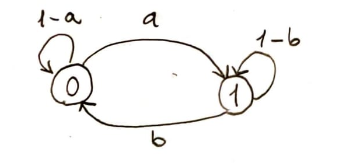
\includegraphics[width=0.5\textwidth]{image004.png}
    \caption{Block diagram for the two-state Markov Chain}
\end{figure}

In this particular case we can compute analytically the $n$-step transition matrix:
\begin{align}
    \textbf{P}^n = \frac{1}{a+b} \left(\begin{array}{cc}
    b & a \\ 
    b & a
    \end{array}\right)  + \frac{(1-a-b)^n}{a+b} \left(\begin{array}{cc}
    a & -a \\ 
    -b & b
    \end{array}\right) \label{eqn:n-matrix}
\end{align}

We can rewrite it in a more compact form by introducing:
\begin{align*}
    \textbf{A} = \left(\begin{array}{cc}
    b & a \\ 
    b & a
    \end{array}\right) \qquad \textbf{B} = \left(\begin{array}{cc}
    a & -a \\ 
    -b & b
    \end{array}\right) 
\end{align*}

So that (\ref{eqn:n-matrix}) becomes:
\begin{align}\label{eqn:n-matrix2}
    \textbf{P}^n = (a+b)^{-1} [\textbf{A} + (1-a-b)^n \textbf{B}]   
\end{align}

\textbf{Proof}. By induction, we start with proving the $n=1$ case, and then show that if (\ref{eqn:n-matrix}) holds up to $n$, then it holds also for $n+1$. Explicitly:
\begin{align*}
    \textbf{P}^1 &= \frac{1}{a+b} \left(\begin{array}{cc}
    b & a \\ 
    b & a
    \end{array}\right) + \frac{1-a-b}{a+b} \left(\begin{array}{cc}
    a & -a \\ 
    -b & b
    \end{array}\right) =\\
    &= \frac{1}{a+b} \left(\begin{array}{cc}
    b+a-a^2-ab & a-a+a^2+ab \\ 
    b-b+ab+b^2 & a+b-ab-b^2
    \end{array}\right) =\\
    &= \frac{1}{a+b} \left(\begin{array}{cc}
    (1-a)(a+b) & a(a+b) \\ 
    b(a+b) & (1-b)(a+b)
    \end{array}\right) =\\
    &= \left(\begin{array}{cc}
    1-a & a \\ 
    b & 1-b
    \end{array}\right) = \textbf{P} 
\end{align*}
For the induction step:
\begin{align*}
    \textbf{P}^{n+1} &= \textbf{P}^n\textbf{P} \underset{(\ref{eqn:n-matrix2})}{=} (a+b)^{-1}[\textbf{A} + (1-a-b)^n \textbf{B}] \textbf{P} 
\end{align*}
Note that:
\begin{align*}
    \textbf{A} \textbf{P} &= \left(\begin{array}{cc}
    b & a \\ 
    b & a
    \end{array}\right)  \times \left(\begin{array}{cc}
    1-a & a \\ 
    b & 1-b
    \end{array}\right) = \left(\begin{array}{cc}
    b & a \\ 
    b & a
    \end{array}\right) = \textbf{A} \\
    \textbf{B}\textbf{P} &= \left(\begin{array}{cc}
    a & -a \\ 
    -b & b
    \end{array}\right) \times \left(\begin{array}{cc}
    1-a & a \\ 
    b & 1-b
    \end{array}\right)  = (1-a-b)\textbf{B} 
\end{align*}
And so:
\begin{align*}
    \textbf{P}^{n+1} &= (a+b)^{-1} [\textbf{A} + (1-a-b)^{n+1} \textbf{B} ] = \textbf{P}^{n+1} \qquad \square 
\end{align*}

We can now use (\ref{eqn:n-matrix}) to study the asymptotic behaviour. Suppose that $|1-a-b|<1$ (always true in the non trivial cases $0<a,b<1$), then $|1-a-b|^n  \xrightarrow[n \to \infty]{}  0$, and:
\begin{align*}
    \lim_{n \to \infty} \textbf{P}^n = \frac{1}{a+b} \left(\begin{array}{cc}
    b & a \\ 
    b & a
    \end{array}\right) 
\end{align*}
Note that the two rows are equal, meaning that the asymptotic probability distribution does not depend on the initial state: the system will be in state $0$ with probability $b/(a+b)$, and in $1$ with $p=a/(a+b)$. In other words, the system \q{forgets} its initial condition. As we will see, this is a typical behaviour for many cases of Markov chains. 

\begin{appr}
    \textbf{Packet transmission and the two-state model}. One possible application of the two-state model is given by modelling the error rate of a packet transition system with memory. Denote with state $0$ the event of a correct transmission, and with $1$ that of an error. Then the average packet error probability is given by:
    \begin{align*}
        P_e = \frac{a}{a+b} 
    \end{align*}
    Another interesting quantity is the mean length of a \textit{burst} of errors, i.e. how long (on average) does the system spend in state $1$. The mean length $L$ of such a sequence of erroneous states is a geometric random variable (in the two-state model), whose average is the inverse of the probability of \textit{moving out of state $1$}:
    \begin{align*}
        \langle L \rangle = \frac{1}{P_{10}} = \frac{1}{b} 
    \end{align*} 
    In a real scenario, we will need to provide redundancy so that the system \textit{can tolerate} $\langle L \rangle$ consecutive errors.
\end{appr}

\subsection{Markov Chains Defined by Independent r.v.}
Let $\xi$ denote a discrete-valued random variable whose possible values are the nonnegative integers and where $\mathbb{P}[\xi_i = i] = a_i \geq 0$ for $i\in \mathbb{N}$, and $\sum_{i=0}^n a_i = 1$. Let $\xi_1, \xi_2, \dots, \xi_n, \dots$ represent independent measurements of $\xi$.

\medskip

We can use that sequence to construct Markov chains.
\begin{enumerate}
    \item We let $X_n = \xi_n$. The probability transition matrix then becomes:
    \begin{align*}
        \textbf{P} = \left(\begin{array}{cccc}
        a_0 & a_1 & a_2 & \cdots \\ 
        a_0 & a_1 & a_2 & \cdots \\ 
        a_0 & a_1 & a_2 & \cdots \\ 
        \vdots & \vdots & \vdots & \ddots
        \end{array}\right) 
    \end{align*}
    All rows are equal because all the $\xi_n$ are independent of each other. 
    \item \textbf{Successive maxima}.  We define $X_n$ to be the maximum value assumed by the first $n$ r.v. $\xi_i$:
    \begin{align*}
        X_n = \max\{\xi_1, \dots, \xi_n\} \qquad n=1,2,\dots
    \end{align*}
    This is a Markov chain. In fact, any future state $X_{n+1}$ is completely determined by the current state $X_n$ and the outcome of the next r.v. $\xi_{n+1}$, which is i.i.d.:
    \begin{align*}
        X_{n+1} = \max\{X_n, \xi_{n+1}\}
    \end{align*}
    The transition probability matrix is then:
    \begin{align*}
        \textbf{P} = \left(\begin{array}{ccccc}
        A_0 & a_1 & a_2 & a_3 & \cdots \\ 
        0 & A_1 & a_2 & a_3 & \cdots \\ 
        0 & 0 & A_2 & a_3 & \cdots \\ 
        0 & 0 & 0 & A_3 & \cdots \\ 
        \vdots & \vdots & \vdots & \vdots & \ddots
        \end{array}\right) 
    \end{align*}
    where $A_k = \sum_{i=0}^k a_k$. %Finish reading
    \item \textbf{Partial sums}. Similarly to the previous example, we define:
    \begin{align*}
        X_n = \xi_1 + \dots + \xi_n \qquad n=1,2,\dots
    \end{align*} 
    with $X_0 \equiv 0$. %Finish
\end{enumerate}

\subsection{One-Dimensional Random Walks}
Consider a particle moving on a line, such that, at any given time, it can only remain in the current state $i$ with probability $r_i$, or move to the neighbouring ones with probability $q_i$ (left) or $p_i$ (right). This process is a special Markov Chain called a \textbf{random walk}, with transition matrix:
\begin{align*}
    \textbf{P} =  \begin{blockarray}{l*{9}{c}}
        \begin{block}{l*{9}{>{\scriptstyle}c<{}}}
            & 0 & 1 & 2 & & i-1 & i & i+1 &\\
        \end{block}
        \begin{block}{>{\scriptstyle}r<{}(*{9}{c})}
            0 & r_0 & p_0 & 0 & \cdots & 0 & 0 & 0 & \cdots \\
            1 & q_1 & r_1 & p_1 & \cdots & 0 & 0 & 0 & \cdots\\
            2 & 0 & q_2 & r_2 & \cdots & 0 & 0 & 0 & \cdots\\
            \vdots &&&&&&&&\\
            i & 0 & 0 & 0 & \cdots & q_i & r_i & p_i & \cdots\\
            \vdots & \vdots & \vdots & \vdots & \vdots & \vdots & \ddots & \ddots & \ddots \\
        \end{block}
    \end{blockarray}
\end{align*} 
To \q{keep the walk going} we need $p_i, q_i > 0$, while $r_i \geq 0$. All rows sum to $1$, meaning that $q_i + r_i + p_i = 1$ $\forall i$.

\begin{appr}
    \textbf{Random walks and games}. Random walks can be used to model games, by identifying the state $i$ with \textit{the player's score} at a given time. If the player wins the next match, their score will go up. Conversely, if they lose, the state will recess. Note that draws can be modelled by the player \textit{remaining} in the same state.
    
    \medskip

    Similarly, the state can model the amount of \textit{resources} available to the player (i.e. wealth, or \q{health points}). If the player runs out of resources, i.e. they reach state $0$, then they lose. Conversely, the same holds for the opponent. So the state with \textit{maximum resources} for the player (i.e. $N$), corresponds to the loss of the opponent. In this situation there are \textit{two} absorbing states. We will study the asymptotic behaviour in the next sections.  
\end{appr}

Suppose we are modelling a game's score with a random walk. States $0$ and $N$ correspond respectively to the player losing or winning, and so they are absorbing states. 
We also suppose that, at each turn, the score always changes.

\medskip

The transition matrix is then given by:
\begin{align*}
    \textbf{P} =  \begin{blockarray}{l*{7}{c}}
        \begin{block}{l*{7}{>{\scriptstyle}c<{}}}
            & 0 & 1 & 2 & 3 & \cdots & N\\
        \end{block}
        \begin{block}{>{\scriptstyle}r<{}(*{7}{c})}
            0 & 1 & 0 & 0 & 0 & \cdots & 0\\
            1 & q & 0 & p & 0 & \cdots & 0\\
            2 & 0 & q & 0 & p & \cdots & 0\\
            \vdots & \vdots & \vdots & \vdots & \vdots & & \vdots\\
            N & 0 & 0 & 0 & 0 & \cdots & 1\\
        \end{block}
    \end{blockarray}
\end{align*}
with $p+q=1$.

\medskip

If the initial state (i.e. initial amount of resources) is $k$, the average time needed to reach one of the absorbing states is:
\begin{align*}
    T = \min\{n \geq 0; X_n \in \{0,N\}\}
\end{align*}
The probability of losing is given by:
\begin{align}\label{eqn:fsa-game}
    u_k = \mathbb{P}[X_t = 0|X_0=k]
\end{align}
To compute it, we can use first-step analysis:
\begin{align*}
    u_k = p u_{k+1} + q u_{k-1} \qquad k=1,\dots, N-1
\end{align*}
Each step can only lead to the next state (with probability $p$) or to the previous state (with probability $q$). If we start at $0$, then the player instantly loses, i.e. $u_0 = 1$. Conversely, $u_N = 0$.

\medskip

To solve the system, we start by rewriting (\ref{eqn:fsa-game}):
\begin{align}\nonumber
    u_k = \textcolor{Red}{(p+q)}u_k = pu_k + qu_k =p u_{k+1} + q u_{k-1}\span \\
    \Rightarrow q\underbrace{(u_k - u_{k-1})}_{x_k} = p (u_{k+1}-u_k) \label{eqn:uk}
\end{align}

Then we change variables, introducing:
\begin{align*}
    x_k \equiv u_k - u_{k-1}
\end{align*}
So that (\ref{eqn:uk}) may be rewritten as:
\begin{align*}
    k&=1 && 0 = p(u_2-u_1) - q(u_1-u_0) = px_2 - qx_1\\
    k&=2 && 0 = p(u_3-u_2) - q(u_2-u_1) = px_3 - qx_2\\
    &\>\>\>\vdots \span \span\\
    k&=N-1 &&0=p(u_N - u_{N-1}) - q(u_{N-1} - u_{N-2}) = px_N - qx_{N-1}
\end{align*}
Note that we can express each $x_{k+1}$ in terms of $x_k$, and substitute the result in the successive equation, leading to:
\begin{align}\label{eqn:xi}
    x_2 = \frac{q}{p} x_1 \Rightarrow x_3 = \frac{q}{p} x_2 = \left(\frac{q}{p} \right)^2 x_1 \Rightarrow \cdots  \Rightarrow x_N = \left(\frac{q}{p} \right)^{N-1} x_{1}
\end{align}
Now we need to \textit{invert} the change of variables. Note that $u_k$ is equal to the sum of the first $k$ $\{x_i\}$, up to a constant: 
\begin{align}
    \sum_{i=1}^k x_i = \sum_{i=1}^k (u_i - u_{i-1}) = u_k - u_0 \underset{(a)}{=}  u_k - 1
\end{align}
where in (a) we used the \textit{first} boundary condition: $u_0 = 1$.

Rearranging:
\begin{align}\label{eqn:uk}
    u_k = 1 + \sum_{i=1}^k x_i \underset{(\ref{eqn:xi})}{=}  1 + x_1 \sum_{i=1}^k \left(\frac{q}{p} \right)^{i-1} = 1 + x_1 \frac{1-(q/p)^{k}}{1-(q/p)} \qquad q \neq p
\end{align}
To compute $x_1$ we use the \textit{second}  boundary condition $u_N = 0$:
\begin{align*}
    u_N = 0 \underset{(\ref{eqn:uk})}{=}  1+ x_1 \frac{1-(q/p)^{N}}{1-(q/p)} \Rightarrow x_1 = - \frac{1-q/p}{1-(q/p)^N} 
\end{align*}
And substituting back in (\ref{eqn:uk}) we arrive to the final result:
\begin{align} \label{eqn:uk-f}
    u_k = 1 - \frac{1-(q/p)^{k}}{\cancel{1-(q/p)}} \frac{\cancel{1-q/p}}{1-(q/p)^N} = \frac{(q/p)^k - (q/p)^N}{1-(q/p)^N} \qquad q \neq p
\end{align}
In the special case of $p=q=1/2$ we go back and directly compute the sum in (\ref{eqn:uk}):
\begin{align*}
    u_k = 1 + x_1 \sum_{i=1}^k 1 = 1 + k x_1 \qquad p = q
\end{align*}
Where $x_1$ is obtained from $u_N = 0$:
\begin{align*}
    u_N = 0 = 1 + N x_1 \Rightarrow x_1 = -\frac{1}{N} 
\end{align*}
So that:
\begin{align*}
    u_k = 1 - \frac{k}{N} = \frac{N - k}{N} 
\end{align*}

In summary, the probability of the player's losing (i.e. reaching state $0$) if the system starts in state $k$ is given by:
\begin{align*}
    u_k &= \begin{dcases}
        (N-k)/N & p = q = 1/2\\
        \frac{(q/p)^k - (q/p)^N}{1-(q/p)^N} & p \neq q 
    \end{dcases} \qquad  k = 1, \dots, N-1\\
    u_0 &= 1\\
    u_N &= 0
\end{align*}

If we fix $k$, a larger $N$ leads to a higher probability of losing $u_k$, as the resources $N-k$ available to the opponent rise. Conversely, for $N$ fixed, $u_k$ vanishes for large $k$.

\medskip

If we let $N \to \infty$ (opponent \q{infinitely rich}, as a casino), then:
\begin{align*}
    u_k  \xrightarrow[N \to \infty]{}  \begin{cases}
        1 & p \leq q\\
        (q/p)^k & p > q
    \end{cases}
\end{align*}
This means that if the player is at a disadvantage ($p < q$), then there they will certainly lose. However, if the player is likely to win each game ($p>q$), then they may (in principle) continue playing indefinitely. However, note that for any finite $k$ there is still a finite non-zero probability of losing nonetheless, equal to $(q/p)^k$, that vanishes for $k \to +\infty$.

Note that the player will certainly lose even if the game is fair ($p=q$). This can be intuitively understood by looking at fig. \ref{fig:random-walk}.

\begin{figure}[htp]
    \centering
    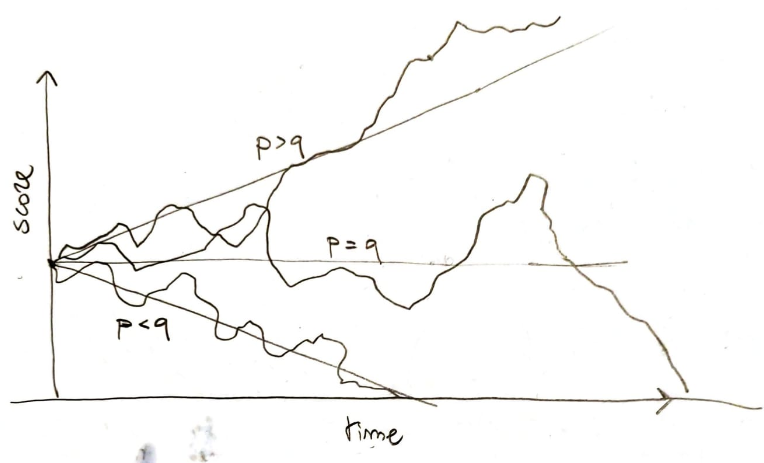
\includegraphics[width=0.8\textwidth]{image005.png}
    \caption{The ratio $p/q$ defines the slope of the \textit{trend} followed by the player's score. If $p/q < 1$, the player will certainly lose after some time. If $p/q=1$ (fair game), the average player's score remains fixed to that of the initial state, and given infinite time a sufficiently high fluctuation will bring the player to ruin. If $p/q > 1$, the player can still lose the game, but on average their score will rise, making their situation \q{safer}.}
\end{figure}

\subsection{Success Runs}
Consider the Markov Chain with the following transition matrix:
\begin{align*}
    \textbf{P} =  \begin{blockarray}{l*{7}{c}}
        \begin{block}{l*{7}{>{\scriptstyle}c<{}}}
            & 0 & 1 & 2 & 3 & 4 & \cdots\\
        \end{block}
        \begin{block}{>{\scriptstyle}r<{}(*{7}{c})}
            0 & p_0 & q_0 & 0 & 0 & 0 & \cdots\\
            1 & p_1 & r_1 & q_1 & 0 & 0 &  \cdots\\
            2 & p_2 & 0 & r_2 & q_2 & 0 & \cdots\\
            3 & p_3 & 0 & 0 & r_3 & q_3 & \cdots \\
            \vdots & \vdots & \vdots & \vdots & \vdots & \vdots & \ddots\\
        \end{block}
    \end{blockarray}
\end{align*}
Starting at state $i$, the system can move to $i+1$ with probability $q_i$, remain at $i$ with probability $r_i$, or \textit{go back to the starting line} at state $0$ with probability $p_i$. 

\begin{figure}[htp]
    \centering
    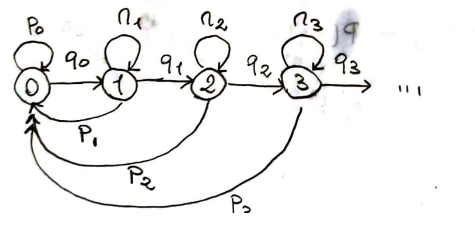
\includegraphics[width=0.6\textwidth]{image006.png}
    \caption{Block diagram for the \textit{success run} Markov Chain \label{fig:success-run}}
\end{figure}

\begin{appr} \textbf{Timeouts}. 
    This kind of chain can be used to model, for example, \textit{timeout processes} - that is processes where a reset happens after a certain time, except when something else prevents it. 
\end{appr}

We apply this kind of model to a \textit{layer $2$} protocol\footnote{Internet works thanks to protocols - a set of shared rules allowing very different machines to \q{communicate} with each other. TCP/IP is one such collection of protocols, which are divided in $4$ \textbf{layers}, representing different kind of \textit{abstractions}. The first layer, which sits at the bottom, is the \textbf{physical layer}, dealing directly with hardware: cables and electronics. The second one is the \textbf{data link layer}, and deals with \textit{subdividing} data in packets, and providing means for error-correction. The following layers allow access to other networks (forming the Internet) and more fancy features such as security, permissions, application specific routing and so on.}, where we want to send \textit{data packets} between \textit{nodes} connected by a \textit{link}. The receiving node confirms the success of transmission by returning an \textit{acknowledgment} message. If this does not happen, the packet needs to be re-transmitted. In practice, this is done for a maximum of $L+1$ total trials (including the first transmission), after which the packet is discarded (otherwise the system would be \textit{clogged} with untransmitted data). 

\medskip

In particular, we denote with $X_n$ the number of \textit{failed transmissions} of a packet. At every state $i < L$, there can be another transmission failure with probability $\epsilon$, leading to state $i+1$, or the packet can be correctly sent with probability $1-\epsilon$, leading to the final state $S$ (success), after which the process stops. If the system reaches $L$ and \textit{fails} one more time, then it will evolve to the final state $F$, where data is discarded, and no more trials are done.   

\medskip

The transition probability matrix is given by:
\begin{align*}
    \textbf{P} =  \begin{blockarray}{l*{9}{c}}
        \begin{block}{l*{9}{>{\scriptstyle}c<{}}}
            & 0 & 1 & 2 & 3 & \cdots & L & F & S\\
        \end{block}
        \begin{block}{>{\scriptstyle}r<{}(*{9}{c})}
            0 & 0 & \epsilon & 0 & 0 & \cdots & 0 & 0 & 1-\epsilon\\
            1 & 0 & 0 & \epsilon & 0 & \cdots & 0 & 0 & 1-\epsilon\\
            2 & 0 & 0 & 0 & \epsilon & \cdots & 0 & 0 & 1-\epsilon\\
            \vdots & \vdots & \vdots & \vdots & \vdots & & \vdots & \vdots & \vdots\\
            L & 0 & 0 & 0 & 0 & \cdots & 0 & \epsilon & 1-\epsilon\\
            F & 0 & 0 & 0 & 0 & \cdots & 0 & 1 & 0\\
            S & 0 & 0 & 0 & 0 & \cdots & 0 & 0 & 1\\
        \end{block}
    \end{blockarray}
\end{align*}

\begin{figure}[htp]
    \centering
    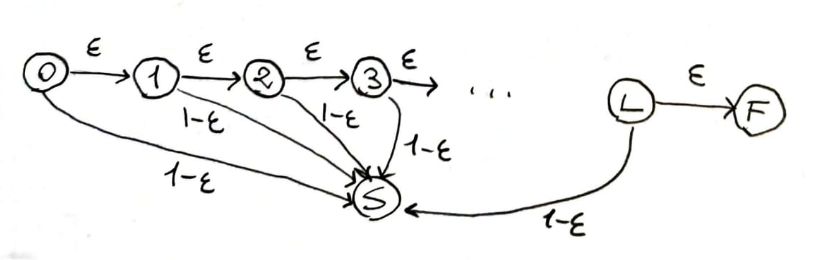
\includegraphics[width=0.8\textwidth]{image007.png}
    \caption{Block diagram for the \textit{layer 2} protocol  \label{fig:layer-two}}
\end{figure}

We are interested in the probability of the chain being absorbed in $S$, given it started in state $i$. This can be computed by first-step analysis:
\begin{align*}
    u_i &= \mathbb{P}[X_T = S|X_0 = i] =\\
    &= \sum_{j=0}^L P_{ij} u_j + P_{iS} \cdot 1 + P_{iF} \cdot 0 = \begin{cases}
        \epsilon u_{i+1} + 1 - \epsilon & i<L\\
        1- \epsilon & i = L
    \end{cases}
\end{align*}
Note that we know $u_L$, and from $u_{i+1}$ we can determine $u_i$. So we can start at the last state, and work our way backwards to the start:
\begin{align*}
    u_0 &= \epsilon u_1 + 1-\epsilon = \epsilon(\epsilon u_2 + 1-\epsilon) + 1 -\epsilon=\\
    &= \epsilon^2 u_2 + (1-\epsilon) \epsilon + (1-\epsilon) = \\
    &= \epsilon^L u_L + \sum_{j=0}^{L-1} \epsilon^j(1-\epsilon)=\\
    &= \epsilon^L (1-\epsilon) + (1-\epsilon) \frac{1-\epsilon^L}{1- \epsilon} = 1 - \epsilon^{L+1} 
\end{align*}
This makes sense, as the probability of having at least a success in $L+1$ trials is equal to the probability of \textit{not} failing $L+1$ consecutive times, which is $1-\epsilon^{L-1}$.

\medskip

The average number of attempts per packet is just the mean time for absorption:
\begin{align*}
    \nu_i = \epsilon v_{i+1} + 1 & i < L
\end{align*}
and $\nu_L = 1$. As before, we iterate:
\begin{align*}
    \nu_0 &= \epsilon \nu_1 + 1 = \epsilon(\epsilon \nu_2 + 1) + 1 = \epsilon^2 \nu_2 + \epsilon + 1=\\
    &= \epsilon^3 \nu_3 + \epsilon^2 + \epsilon + 1 = \epsilon^L \nu_L + \sum_{j=0}^{L-1} \epsilon^j = \\
    &= \epsilon^L + \frac{1-\epsilon^L}{1- \epsilon} = \frac{\cancel{\epsilon^L }- \epsilon^{L+1} + 1 \cancel{- \epsilon^L}}{1-\epsilon} = \frac{1-\epsilon^{L+1}}{1-\epsilon}   
\end{align*}

Let's consider a sequence of transmissions. Each packet has a probability $u_0 = 1- \epsilon^{L+1}$ of being correctly sent, and so the average number of packets sent is $u_0$.
The mean sending time is $\nu_0 = (1-\epsilon^{L+1})/(1-\epsilon)$. The ratio of these two averages is the mean \textbf{throughput} of the channel:
\begin{align*}
    \text{Throughput} = \frac{u_0}{\nu_0} = 1-\epsilon 
\end{align*} 
We will prove this \textit{intuitive} result in a later section.  

\subsection{First Passage Times}
We define the first passage time $\theta_{ij}$ from state $i$ to $j$ as the number of transmissions to reach $j$ from $i$ for the first time. Its distribution is given by:
\begin{align*}
    \mathbb{P}[\theta_{ij} = u] = f_{ij}(u) = \mathbb{P}[X_n = j, X_m \neq j, m=1,\dots, n-1|X_0 = i]
\end{align*}
Note that we are interested in events where $j$ is the last state, and it has not been visited before. So, in other words, $\theta_{ij}$ is the number of transitions from $i$ to states \textit{different} from $j$ needed to reach $j$ for the first time. 

We then define $f_{ij}(0) \equiv 0$ $\forall i \neq j$, as the probability of reaching $j$ from a different state \textit{without moving} is obviously null.

\medskip

We can compute $f_{ij}$ by \textbf{first-step analysis}:
\begin{align}
    f_{ij}(n) = P_{ij} \delta(n-1) + \sum_{i \neq j}P_{ik} f_{kj}(n-1) \qquad \delta(n) = \begin{cases}
        1 & n = 0\\
        0 & n \neq 0
    \end{cases} \label{eqn:fij}
\end{align}
In fact, $f_{ij}$ is $P_{ij}$ if $n=1$, i.e. if we are asking the probability of $i \to j$ in one step. Otherwise, the system has to go to a different state $k \neq i$ (with probability $P_{ik}$), where the first passage time to $j$ becomes $f_{kj}(n-1)$ (as we have done already a step). By reiterating (\ref{eqn:fij}) we can express $f_{ij}(n)$, for any $n$, as a only a function of \textbf{P}.

\medskip

For example, let's do this for the two-state chain, where the transition matrix is:
\begin{align*}
    \textbf{P} = \left(\begin{array}{cc}
    1-a & a \\ 
    b & 1-b
    \end{array}\right)
\end{align*}
Suppose the system starts at $0$, and we are interested in the first passage time to $1$. Expanding (\ref{eqn:fij}) leads to:
\begin{align*}
    f_{01}(n) &= P_{01} \delta(n-1) + P_{00} f_{01}(n-1) = \begin{cases}
        a & n=1\\
        (1-a) f_{01}(n-1) & n > 1
    \end{cases}
\end{align*}
Then:
\begin{align} \nonumber
    f_{01}(2) &= a(1-a)\\  \nonumber
    f_{01}(3) &= a (1-a)^2\\
    \Rightarrow f_{01}(n) &= (1-a)^{n-1} a \qquad n\geq 1
    \label{eqn:f01}
\end{align}
Similarly:
\begin{align*}
    f_{11}(n) &= P_{11} \delta(n-1) + P_{10} f_{01}(n-1) =\\
    &= (1-b) \delta(n-1) + b f_{01}(n-1) \underset{(\ref{eqn:f01})}{=}  \begin{cases}
        1 - b & n=1\\
        a b (1-a)^{n-2} & n>1
    \end{cases}
\end{align*}
And we can compute $f_{10}$ and $f_{00}$ by substituting $a \leftrightarrow b$ in $f_{01}$ and $f_{11}$ (by symmetry).

\medskip

All these results are rather obvious in the case of the two-state model, as they can be computed by using the geometric distribution. For example, $f_{10}(n)$ is equal to the probability of reaching $0$ from $1$ after exactly $n$ steps, which is equivalent to the probability of \textit{not leaving} $0$ for $n-1$ steps (which is $(1-a)^{n-1}$), and then leaving it on the last step (which is $a$). 

Similarly, for $f_{11}(n)$ we first need to move to $0$ (probability $a$), remain there for $n-2$ steps (probability $(1-a)^{n-2}$) and finally return to $0$ (probability $b$). Clearly, this kind of explicit reasoning is only possible in this case, because there are only two states. In a general situation, first-step analysis is required.

\medskip

First passage times are closely related with \textbf{multi-step transition probabilities}.\marginpar{2. Multi-step transition probabilities} For example, suppose we are interested in the probability of finding a process in state $j$ after $n$ steps, given it started at state $X_0 =i$.

We can then consider all the paths that reach $j$ for the first time in $m \leq n$ steps, and then transition from $j$ to $j$ in the remaining $m-n$ steps. Note that all these paths are \textit{disjoint} events, as each path can reach $j$ for the \textbf{first} time only once!

Then:
\begin{align*}
    P_{ij}^{(n)} = \sum_{m=1}^n f_{ij}(m) P_{jj}^{(n-m)} \qquad n \geq 1
\end{align*}
As we know $P_{ij}^{(n)}$ for any $n$ from \textbf{P}, we can then compute $f_{ij}(m)$ by solving a system of $n$ equations.

\medskip

We can make the problem a bit simpler by highlighting the last term in the sum:
\begin{align*}
    P_{ij}^{(n)} = \sum_{m=1}^{n\textcolor{red}{-1}} f_{ij}(m) P_{jj}^{(n-m)} + \textcolor{Red}{f_{ij}(n)}
\end{align*}
Rearranging:
\begin{align*}
    f_{ij}(n) = \begin{cases}
        0 & n = 0\\
        P_{ij} & n = 1\\
        P_{ij}^{(n)} - \sum_{m=1}^{n-1} f_{ij}(m) P_{jj}^{(n-m)} & n \geq 2
    \end{cases}
\end{align*}
which can be solved by recursion.

\medskip

Note that computing $f_{ij}(n)$ in this way does not require $f_{kj}(m)$ $\forall m < n$ and $\forall k \neq j$ (unlike the first-step analysis method), but only $f_{ij}(m)$ $\forall m < n$.However, we need all powers $\textbf{P}^m$ for $m < n$. So, at the end, the computational complexity is of the same order.  

\medskip

Often, however, we are interested\marginpar{Moments} merely in the moments of $\theta_{ij}$, and not in the full statistics $f_{ij}$. We start by noting that:
\begin{align}\label{eqn:theta-prob}
    \theta_{ij} = \begin{cases}
        1 & \text{with prob. $P_{ij}$}\\
        1+ \theta_{kj} & \text{with prob. $P_{ik}$, $k\neq j$}
    \end{cases}
\end{align}
In fact, if we reach $j$ in only one step (which happens with probability $P_{ij}$), then $\theta_{ij} = 1$. Otherwise, with probability $P_{ik}$ we will travel to another state $k \neq j$, meaning that the first passage time $i \to j$ will be $1$ (as we already did a step) plus the number $\theta_{kj}$ of \textit{steps} yet to make from $k$. 

\medskip

Averaging both sides of (\ref{eqn:theta-prob}) leads to:
\begin{align}\nonumber
    \mathbb{E}[\theta_{ij}] &= P_{ij} + \sum_{k \neq j}^N P_{ik} ( 1 + \mathbb{E}[\theta_{kj}]) =\\ \nonumber
    &= \underbrace{\sum_{k=0}^N P_{ik}}_{1}  + \sum_{k\neq j}^N \mathbb{E}[\theta_{kj}] = \\
    &\underset{(a)}{=}  1+ \sum_{k \neq j}^N P_{ik} \mathbb{E}[\theta_{kj}] \qquad \forall i, j \label{eqn:reflexive}
\end{align}
where in (a) we used the fact that all rows of \textbf{P} sum to $1$ due to normalization.  

\medskip

For a fixed $j$, we have $N+1$ possible values for $i$, so we can write $N+1$ independent equations. These can then be solved to determine all the $\mathbb{E}[\theta_{ij}]$. More precisely, note that $\mathbb{E}[\theta_{jj}]$ does not appear in the rhs of (\ref{eqn:reflexive}), and so we have only $N$ equations to solve:
\begin{align*}
    \mathbb{E}[\theta_{ij}] = 1+ \sum_{k \neq j} P_{ik} \mathbb{E}[\theta_{kj}] \qquad i \neq j
\end{align*}
After having found all the $\mathbb{E}[\theta_{ij}]$ for $i=0, \dots, N$ and $i\neq j$, we can then compute:
\begin{align*}
    \mathbb{E}[\theta_{jj}] = 1 + \sum_{k \neq j} P_{ik} \mathbb{E}[\theta_{kj}]
\end{align*}

\medskip

For example, in the two-state model we have:
\begin{align*}
    \mathbb{E}[\theta_{01}] &= 1 + P_{00} \mathbb{E}[\theta_{01}] \Rightarrow \mathbb{E}[\theta_{01}] = \frac{1}{1 - P_{00}} = \frac{1}{a}\\
    \mathbb{E}[\theta_{10}] &= 1 + P_{11} \mathbb{E}[\theta_{10}] \Rightarrow \mathbb{E}[\theta_{10}] = \frac{1}{1- P_{11}} = \frac{1}{b}
\end{align*}
And then we can compute the cases with $i=j$:
\begin{align*}
    \mathbb{E}[\theta_{00}] &= 1+ P_{01} \mathbb{E}[\theta_{10}] = 1 + \frac{a}{b} = \frac{a+b}{b} = \left(\frac{b}{a+b} \right)^{-1}\\
    \mathbb{E}[\theta_{11}] &= 1+P_{10} \mathbb{E}[\theta_{01}] = 1 + \frac{b}{a} = \frac{a+b}{a} = \left(\frac{a}{a+b} \right)^{-1}
\end{align*}
Note that $\mathbb{E}[\theta_{00}]$ and $\mathbb{E}[\theta_{11}]$ are the reciprocals of the long-run probabilities of remaining respectively in state $0$ or $1$. Intuitively, if the system returns from state $0$ to state $0$ after, on average, $(a+b)/b$ time units, then the fraction of time spent on state $0$ is the inverse of that quantity - because the systems visit $0$ \q{once every $\mathbb{E}[\theta_{00}]$} steps. This kind of result is actually a property of many Markov Chains, as we will see in a later section.


\medskip

For \textbf{second moments} we have:
\begin{align*}
    \mathbb{E}[\theta_{ij}^2] &= P_{ij} \cdot 1^2 + \sum_{k \neq j}^N P_{ik} \mathbb{E}[(1+ \theta_{kj})^2] =\\
    \shortintertext{Expanding the square:}
    &= \underbrace{P_{ij} + \sum_{k \neq j}^N P_{ik}}_{1} + 2 \sum_{k\neq j}^N P_{ik} \mathbb{E}[\theta_{kj}] + \sum_{k \neq j}^N P_{ik} \mathbb{E}[\theta_{kj}^2] =\\
    &\underset{(\ref{eqn:reflexive})}{=}  1 + 2(\mathbb{E}[\theta_{ij}]-1) + \sum_{k \neq j}^N P_{ik} \mathbb{E}[\theta_{kj}^2] =\\
    &= 2 \mathbb{E}[\theta_{ij}] - 1 + \sum_{k \neq j} P_{ik} \mathbb{E}[\theta_{kj}^2]
\end{align*} 
In the two-state case this becomes:
\begin{align*}
    \mathbb{E}[\theta_{01}^2] = 2 \mathbb{E}[\theta_{01}] - 1 + P_{00} \mathbb{E}[\theta_{01}^2] \Rightarrow \mathbb{E}[\theta_{01}^2] = \frac{2 \mathbb{E}[\theta_{01}]-1}{1- P_{00}} = \frac{2/a - 1}{a} = \frac{2}{a^2} - \frac{1}{a}  
\end{align*}
And so:
\begin{align*}
    \operatorname{Var}(\theta_{01}) = \frac{1-a}{a^2}  
\end{align*}
which is exactly the same result we could get by reasoning with the geometric distribution.

Similarly:
\begin{align*}
    \mathbb{E}[\theta_{01}^2] = 2 \mathbb{E}[\theta_{10}] - 1 + P_{11} \mathbb{E}[\theta_{10}^2] \Rightarrow \operatorname{Var}(\theta_{10})  = \frac{1-b}{b} 
\end{align*}
For the $i=j$ case we have, for example:
\begin{align*}
    \mathbb{E}[\theta_{00}^2] &= 2\mathbb{E}[\theta_{00}] - 1 + P_{01} \mathbb{E}[\theta_{10}^2] = 2\left(1 + \frac{a}{b} \right) -1 + a\left(\frac{2}{b^2}-\frac{1}{b}  \right) =\\
    &= 1 +\frac{a}{b} +\frac{2a}{b^2} \\
    \operatorname{Var}(\theta_{00}) &= \mathbb{E}[\theta_{00}^2] - \mathbb{E}[\theta_{00}]^2 =  1 + \frac{a}{b} + \frac{2a}{b^2} - \left(1 + \frac{2a}{b} + \frac{a^2}{b^2}  \right)  =\\
    &= \frac{2a - a^2}{b^2} - \frac{a}{b} = \frac{a(2-a-b)}{b^2}   
\end{align*}


\end{document}

